\chapter{Базовые регрессионные модели и оценка качества}

\section{Обучение базовых регрессоров}

Согласно пункту 2 задания были обучены три базовые модели со стандартными гиперпараметрами:
\begin{enumerate}
    \item \textbf{LinearRegression} — метод наименьших квадратов (МНК) без регуляризации:
    \begin{equation}
        \min_{w, w_0} \frac{1}{2n} \sum_{i=1}^n \left( y_i - w_0 - \sum_{j=1}^m w_j x_{ij} \right)^2
    \end{equation}
    \item \textbf{Lasso} — линейная регрессия с $L_1$-штрафом при стандартном параметре силы $\alpha = 1.0$:
    \begin{equation}
        \min_{w, w_0} \frac{1}{2n} \|y - Xw - w_0\|_2^2 + \alpha \|w\|_1
    \end{equation}
    \item \textbf{ElasticNet} — модель с комбинированным штрафом при $\alpha = 1.0$ и $l_1\text{-ratio} = 0.5$:
    \begin{equation}
        \min_{w, w_0} \frac{1}{2n} \|y - Xw - w_0\|_2^2 + \alpha \cdot l_1 \|w\|_1 + \frac{\alpha (1 - l_1)}{2} \|w\|_2^2
    \end{equation}
\end{enumerate}

\begin{lstlisting}[language=Python]
from sklearn.linear_model import LinearRegression, Lasso, ElasticNet

model_lr = LinearRegression().fit(X_train_scaled, y_train)
model_lasso = Lasso(random_state=42).fit(X_train_scaled, y_train)
model_elastic = ElasticNet(random_state=42).fit(X_train_scaled, y_train)
\end{lstlisting}

\section{Метрики качества на тестовой выборке}

Оценка производительности на 500 объектах тестовой выборки проведена по четырем ключевым метрикам: среднеквадратичной ошибке ($MSE$), корню из нее ($RMSE$), средней абсолютной ошибке ($MAE$) и коэффициенту детерминации ($R^2$).

\begin{table}[H]
\centering
\small
\caption{Сравнение метрик качества базовых моделей регрессии}
\resizebox{\textwidth}{!}{
\begin{tabular}{|l|c|c|c|c|}
\hline
\textbf{Модель} & \textbf{MSE} & \textbf{RMSE (млн EGP)} & \textbf{MAE (млн EGP)} & \textbf{$R^2$} \\
\hline
LinearRegression & $5.96 \times 10^{12}$ & 2.441 & 1.794 & 0.8242 \\
Lasso ($\alpha=1.0$) & $5.96 \times 10^{12}$ & 2.441 & 1.794 & 0.8242 \\
ElasticNet ($\alpha=1.0$) & $1.21 \times 10^{13}$ & 3.483 & 2.477 & 0.6380 \\
\hline
\end{tabular}
}
\end{table}

\section{Анализ предсказаний и распределения весов}

На рисунке 1 приведены диаграммы рассеяния прогнозов базовых моделей относительно фактических цен объектов.

\begin{figure}[H]
    \centering
    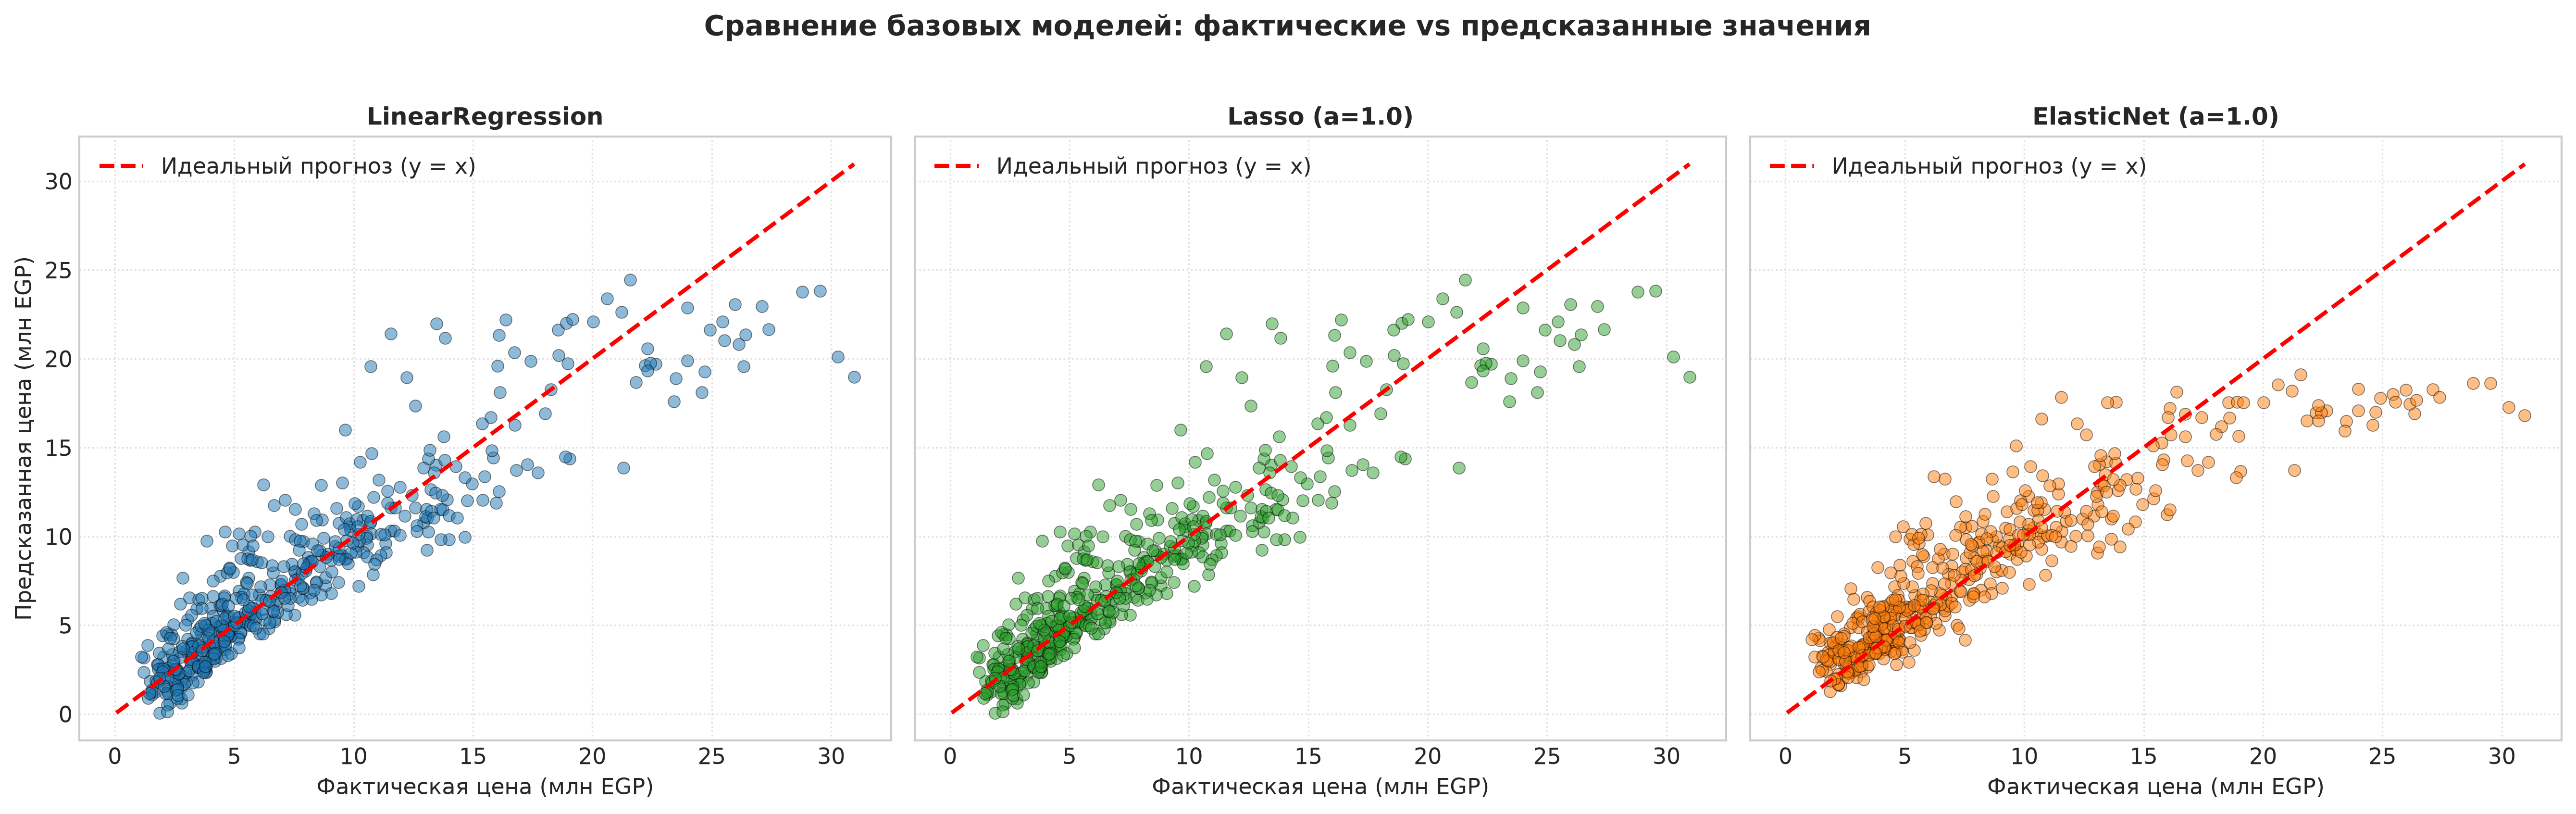
\includegraphics[width=\textwidth]{actual_vs_predicted_baseline.png}
    \caption{Сравнение базовых моделей: фактические vs предсказанные значения}
\end{figure}

Диаграмма наглядно демонстрирует, что точки прогнозов LinearRegression и Lasso плотно концентрируются вокруг диагональной линии идеального совпадения $y = x$. Напротив, базовый ElasticNet систематически занижает стоимость дорогих объектов (более 15 млн фунтов), что приводит к веерообразному отклонению облака точек.

На рисунке 2 сопоставлены численные значения коэффициентов признаков.

\begin{figure}[H]
    \centering
    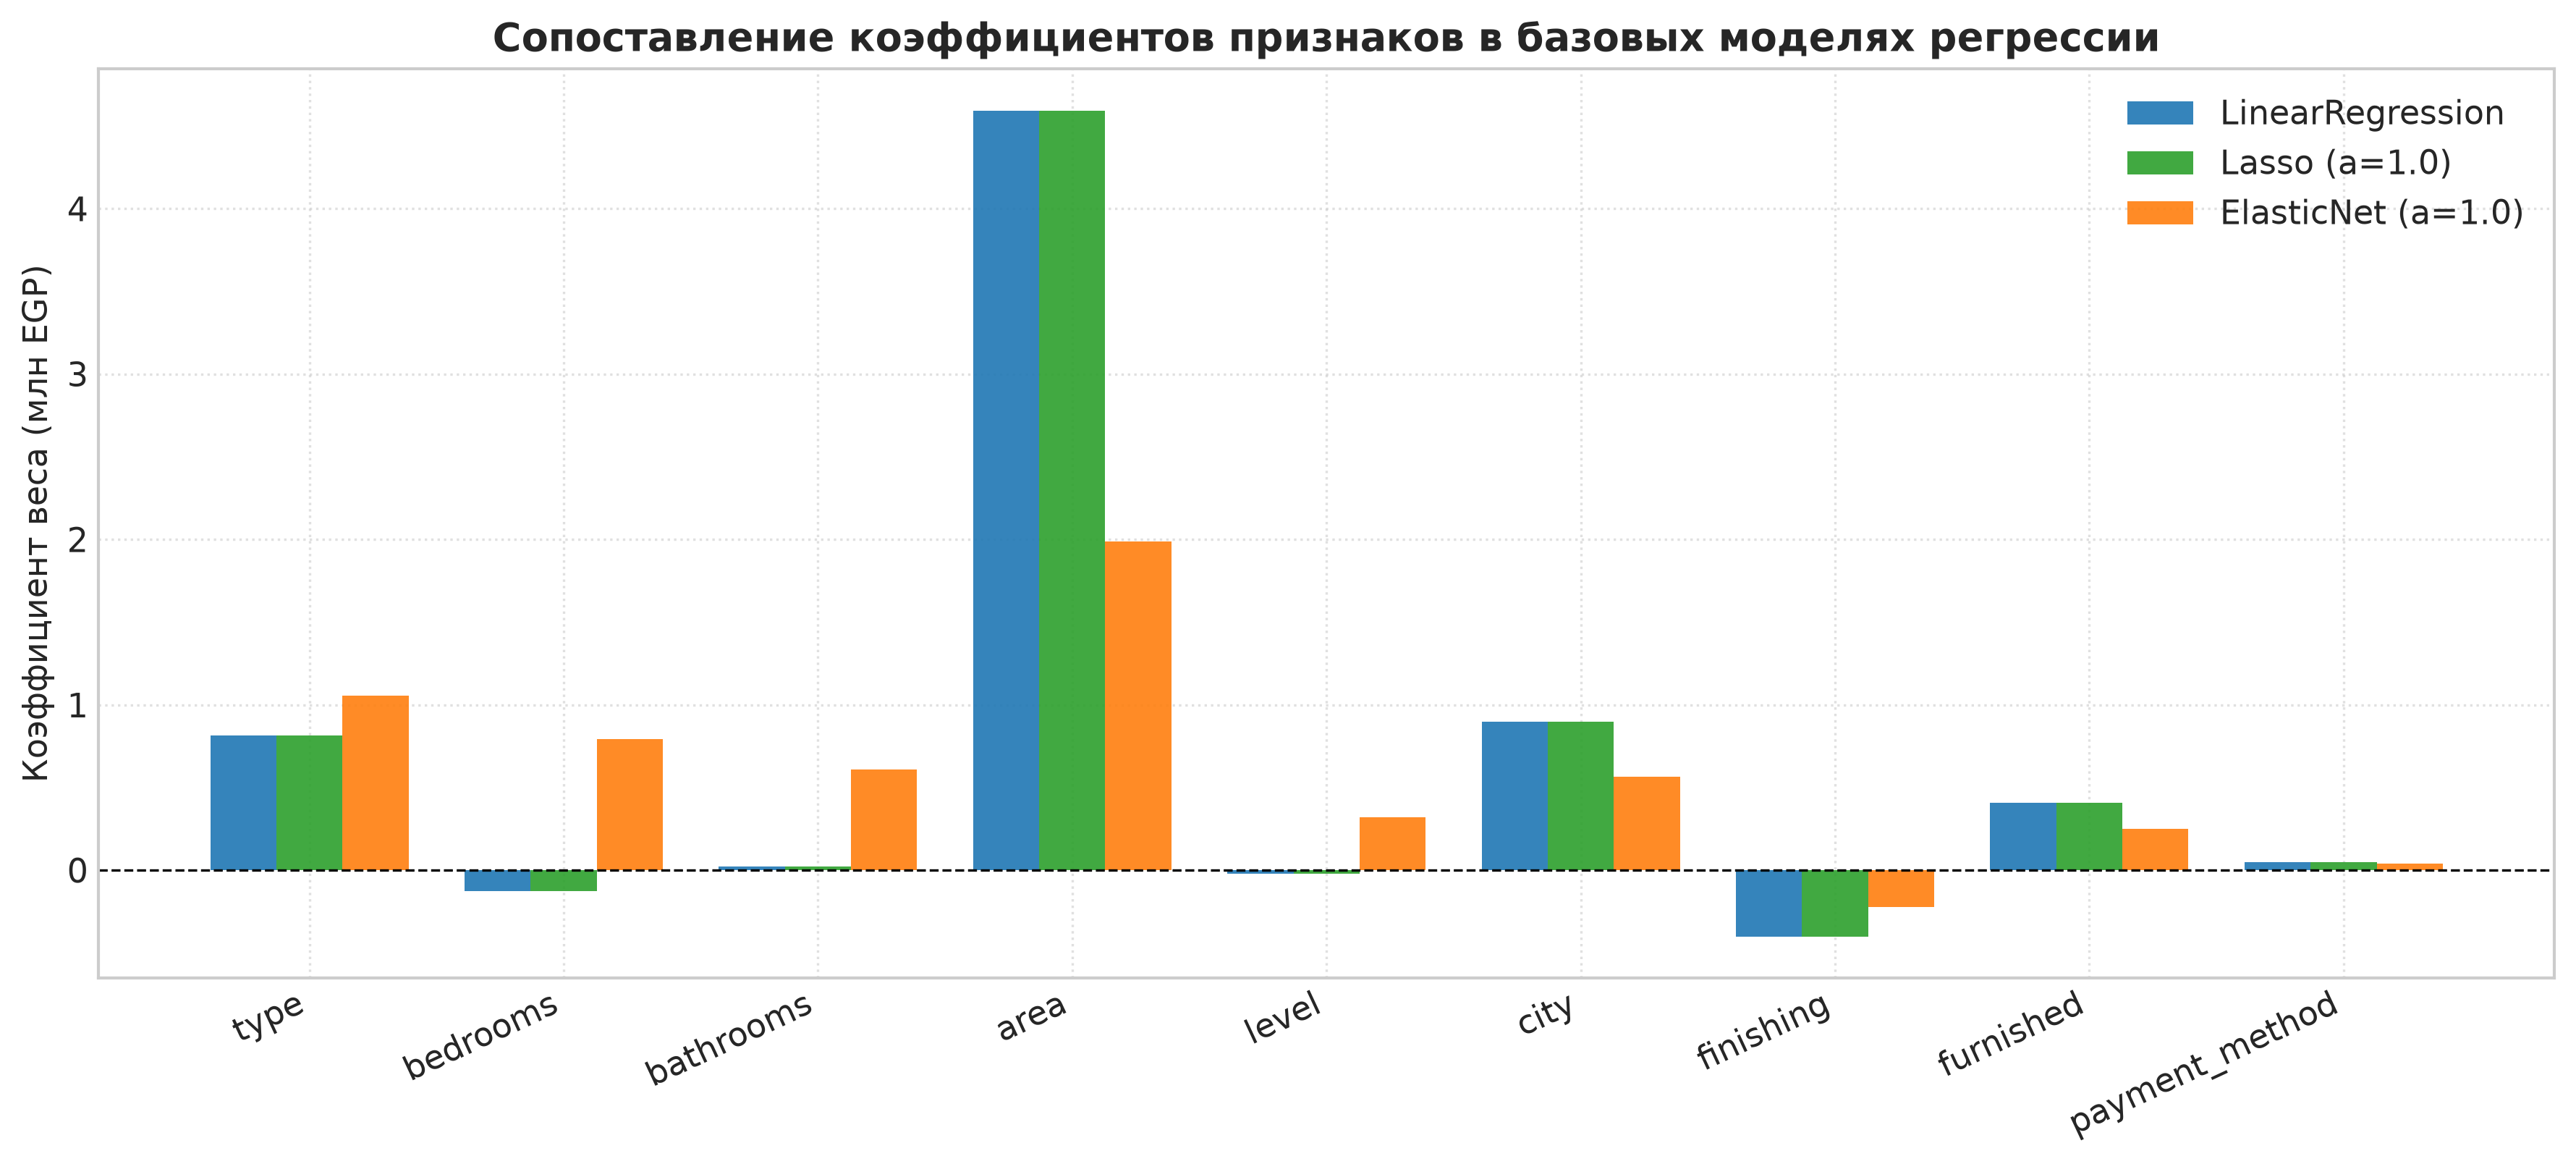
\includegraphics[width=\textwidth]{coefficients_comparison_baseline.png}
    \caption{Сопоставление коэффициентов признаков в базовых моделях}
\end{figure}

\begin{table}[H]
\centering
\caption{Веса признаков в базовых регрессорах (в млн EGP)}
\begin{tabular}{|l|c|c|c|}
\hline
\textbf{Признак} & \textbf{LinearRegression} & \textbf{Lasso} & \textbf{ElasticNet} \\
\hline
\texttt{type} & +0.768 & +0.768 & +0.655 \\
\texttt{bedrooms} & +0.814 & +0.814 & +0.781 \\
\texttt{bathrooms} & +0.339 & +0.339 & +0.552 \\
\texttt{area} & +5.163 & +5.163 & +2.234 \\
\texttt{level} & -0.063 & -0.063 & +0.024 \\
\texttt{city} & +0.222 & +0.222 & +0.207 \\
\texttt{finishing} & -0.198 & -0.198 & -0.138 \\
\texttt{furnished} & +0.165 & +0.165 & +0.178 \\
\texttt{payment\_method} & +0.640 & +0.640 & +0.407 \\
\hline
\end{tabular}
\end{table}

\section{Выводы по разделу 2}

МНК и базовый Lasso с единичным коэффициентом $\alpha=1.0$ выдали совпадающие результаты. Причиной служит масштаб значений: средняя цена квартиры составляет миллионы фунтов, поэтому штраф $\alpha=1.0$ пренебрежимо мал по сравнению с функцией потерь и не производит отбора признаков.

Базовый ElasticNet с теми же параметрами резко просел по точности ($R^2$ упал с 0.82 до 0.64). На диаграмме весов видно, что штраф $L_2$ искусственно занизил вес доминирующего фактора площади (\texttt{area}) более чем в два раза — с 5.16 до 2.23 млн фунтов. Это экспериментально подтверждает недопустимость использования регуляризованных моделей со стандартными параметрами без их калибровки под масштаб конкретной задачи.
